
\ifintegriereaufgaben

\section*{Integrierbare Funktionen Aufgaben}\label{MA2-integrierbare-funktionen-aufgaben}
Erkl�rungen und Beispiele, die zur Bearbeitung der Aufgaben hilfreich sind, finden Sie im Skript\wennreferenzvorhanden{MA2-integrierbare-funktionen}{ (Abschnitt \abschnittsverweis{MA2-integrierbare-funktionen})} und, falls Sie nicht weiterkommen, schauen Sie \hyperref[MA2-integrierbare-funktionen-loesungen]{hier}.
\else
\section{Integrierbare Funktionen Aufgaben}\label{MA2-integrierbare-funktionen-aufgaben}

Regeln und Beispiele zu diesen Aufgaben finden Sie im Skript. Die L�sungen finden Sie \hyperref[MA2-integrierbare-funktionen-loesungen]{hier}.
\fi

\begin{exercisebox}[Gram-Schmidtsches Orthogonalisierungsverfahren]
	Gegeben sind drei linear unabh�ngige Vektoren. Bestimmen Sie ein Orthonormalsystem.
	\[
		\boldsymbol v_1 = \left( \begin{array}{c} 1 \\ i \\ 0 \\ 0 \end{array}\right)\,,
		\boldsymbol v_2 = \left( \begin{array}{c} i \\ 0 \\ 0 \\ i \end{array}\right)\,,
		\boldsymbol v_3 = \left( \begin{array}{c} 1 \\ 0 \\ 1 \\ 0 \end{array}\right)\,.
	\]
\end{exercisebox}

\begin{exercisebox}[Basis] %https://www.lntwww.de/Aufgaben:Aufgabe_4.1:_Zum_Gram-Schmidt-Verfahren
	Bei der Digitalsignal�bertragung werden energiebegrenzte Signale betrachtet. Das Skalarprodukt zweier Signale bzw. die Norm eines Signals sind hierbei wie folgt definiert:
	\begin{eqnarray*}
		\langle s_i, s_k\rangle &=& \int\limits_{-\infty}^{\infty} s_i(t) \cdot s_k(t) \, \mathrm{d}t\,,\\[1ex]
		\|s\| &=& \sqrt{\langle s,s \rangle}\,.
	\end{eqnarray*}
	Betrachten Sie die folgenden drei energiebegrenzten Signale:
	\begin{center}
	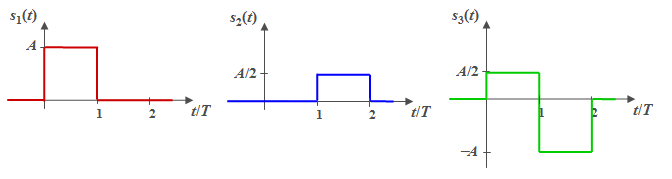
\includegraphics[width=0.7\textwidth]{../Mathematik_2/Bilder/funktionenraum_rechtecksignale_linearkombination.png}
\end{center}
	\begin{itemize}
		\item[(a)] Wie lauten die Abbildungsvorschriften der Signale $s_1, s_2$ und $s_3$?
		\item[(b)] Berechnen Sie die Normen der Signale $s_1$ und $s_2$.
		\item[(c)] Konstruieren Sie aus den Signalen $s_1$ und $s_2$ ein Orthonormalsystem.
		\item[(d)] Zerlegen Sie das Signal $s_3$ bez�glich des Orthonormalsystems und bestimmen Sie die vektoriellen Repr�sentanten der Ausgangssignale bez�glich des Orthonormalsystems.
	\end{itemize}
\end{exercisebox}

\begin{exercisebox}[Orthogonalit�tsrelationen]
	Berechnen Sie f�r alle $k,l\in\mathbb N_0$ mit $\omega = 2\pi/T$ die folgenden Integrale:
	\begin{eqnarray*}
		(a)\, \int\limits_{0}^{T} \cos(k\omega t) \cdot \cos(l\omega t)\, \mathrm{d}t\,, \quad (b)\, \int\limits_{0}^{T} \sin(k\omega t) \cdot \sin(l\omega t)\, \mathrm{d}t\,,\quad (c)\, \int\limits_{0}^{T} \cos(k\omega t) \cdot \sin(l\omega t)\, \mathrm{d}t
	\end{eqnarray*}
\end{exercisebox}


